\subsection{The Cherenkov Telescope Array}\label{sec:CTA}
%%%%%%%%%%%%%%%%%%
The \CTAO will represent the next generation of imaging atmospheric Cherenkov telescopes (IACTs), improving the technology of the current ground-based $\gamma$-ray detectors, such as H.E.S.S., MAGIC, and VERITAS. It is designed to surpass the sensitivity of current IACTs by an order of magnitude in the TeV regime, to improve the angular resolution, as well as to enhance the surveying and monitoring capabilities. CTAO  will consist of two IACT arrays: one located in the Southern hemisphere (CTAO-South) and the other in the Northern hemisphere (CTAO-North) \cite{CTAConsortium:2017dvg}.

The configuration will use three different types of telescope: large-, medium-, and small-sized telescopes (LST, MST, and SST, respectively), detecting photons over a broad energy range from 20 GeV up to 300 TeV. The LSTs will be most sensitive at lower energies, while the SSTs will cover the highest energies. The SSTs will be {dedicated primarily to the observation of}  phenomena occurring within our Galaxy and will {therefore be deployed only at the southern site from which} the central/inner part of the Galaxy is most visible. LSTs and MSTs will instead be built both in the Northern and Southern locations and will focus on observations of extragalactic targets.

The telescopes will be equipped with cameras featuring wide fields of view: 
{4.3$^\circ$} for LSTs, {7.5--7.7$^\circ$} for MSTs, and {8.8$^\circ$} for SSTs. A wide field of view is important for observing extended sources and diffuse emission, as well as for reducing the systematic errors of the measurements when requiring a uniform response over regions much larger than the telescope point-spread function (PSF). Several surveys covering large portions of the sky are planned as part of CTAO's observational strategy, and will be performed as Key Science Projects (KSPs) of the observatory early in the observatory's operation 
\cite{CTAConsortium:2017dvg}. Thanks to its improved sensitivity and wider field of view, {CTAO will surpass} the surveying capabilities of existing IACTs. In particular, the Extra-Galactic survey (detailed below) { will be} the largest survey ever undertaken by IACTs.   

At the same time, CTAO will carry out a large number of traditional, dedicated pointings across the sky. The off-source data collected through these observations will cumulatively cover a substantial sky area with a significant average exposure. In this work, we consider extragalactic data obtained from both observational strategies, as detailed in two subsections below.

\subsubsection{The Extra-Galactic survey}

To study the auto- and cross-correlation signals with gamma-rays, {it is essential to use maps of large sky regions with approximately uniform coverage}. Among CTAO Key Science Projects, the dedicated survey of the extragalactic sky---referred to as the extra-galactic (EGAL) survey - presents the required characteristics.

As described in \cite{CTAConsortium:2017dvg} (Sect. 8), the EGAL survey will cover a quarter of the sky, targeting the region defined by Galactic coordinates $-90^\circ < l < 90^\circ$ and $b > 5^\circ$. The survey is planned to reach an integral sensitivity $\sim$ 6 mCrab above 125 GeV. One of its main objectives is to provide a high-resolution map of the extragalactic sky for photons with energies at least up to 10 TeV and to compile a catalog of very high energy (VHE) extragalactic sources.

The EGAL observations are planned to be carried out over three years of observations, using the full CTAO Observatory (both the Southern and Northern arrays) to achieve nearly uniform sensitivity over the survey region. It is proposed that 15\% of the sky will be covered by the Southern array using 400 h and 10\% by the Northern array using 600 h, resulting in a total observation time of $\sim$ 1000 h. The default {observing strategy consists of a grid spaced by $\sim 3^\circ$ across the survey area, with each pointing observed for 0.51 h in the South and 1.11 h in the North. This configuration is expected to yield an effective exposure of approximately 3 h per point within the EGAL survey boundary.} 

\subsubsection{Simulating survey observations}
To simulate the planned EGAL survey observations, we use the software package \texttt{ctools},\footnote{\url{http://CTA.irap.omp.eu/ctools/}.} developed for a scientific analysis of CTA data. 
We used the instrument response functions (IRFs) for the observatory,\footnote{See \url{http://www.CTA-observatory.org/science/CTA-performance/} for more details.} labeled \texttt{prod3b-v2}, defining the so-called ``omega'' configuration. The respective IRF data files are publicly available at Ref. \cite{zenodo_ctao}.

To enclose the region of the sky covered by the EGAL survey, we simulate observations using telescope-pointing directions corresponding to a HealPix realization with \texttt{NSIDE} = 16, resulting in 694 (3072) pointings within the EGAL survey bounds (over the whole sky). With this setup, the typical angular separation between adjacent pointings is $\sim 3.7^\circ$. {For definiteness,} the radius of the field of view (FoV) of each pointing is set to $6^\circ$. The pointing directions used for the simulation of the EGAL survey within the region of interest (ROI) are shown in \cref{fig:pnts}.

\begin{figure}[t!]
    \centering
    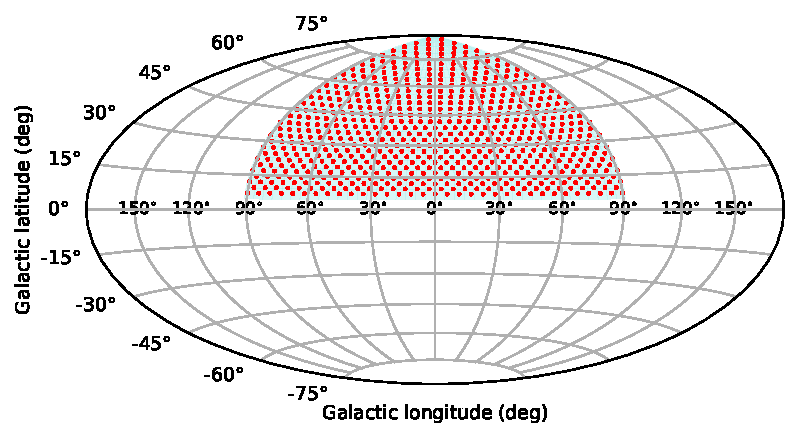
\includegraphics[width=0.45\textwidth]{paper_xcorr/figures/previous_analysis/pointings_NSIDE16.pdf}
    \caption{Pointing directions for the region of the sky {planned to be covered by the extragalactic survey. The pointing directions are shown using a HEALPix pixelization with NSIDE = 16.}}
    \label{fig:pnts}
\end{figure}

The overlap of the FoV from different pointings contributes to a more uniform coverage of the survey’s ROI, minimizing the fluctuations in the exposure that inevitably occur when smaller FoV observations are used to cover a large survey area. Depending on the selected \texttt{HealPix} grid size (i.e., the values of the \texttt{NSIDE} parameter) and the pointing radius for individual observations, the overlap between nearby pointings can vary in extent. The overlaps between pointings are schematically shown in \cref{fig:pnt_zoom}, where the upper panel presents a zoomed-in scheme of the pointing strategy from \cref{fig:pnts}, and the bottom panel shows the simulated exposure of the same region. These images demonstrate that the overlap of nearby pointings creates an anisotropy pattern in the corresponding observation exposure, with variations of approximately $\sim10\%$ relative to the average exposure within the plotted region.

\begin{figure}[t!]
    \centering
    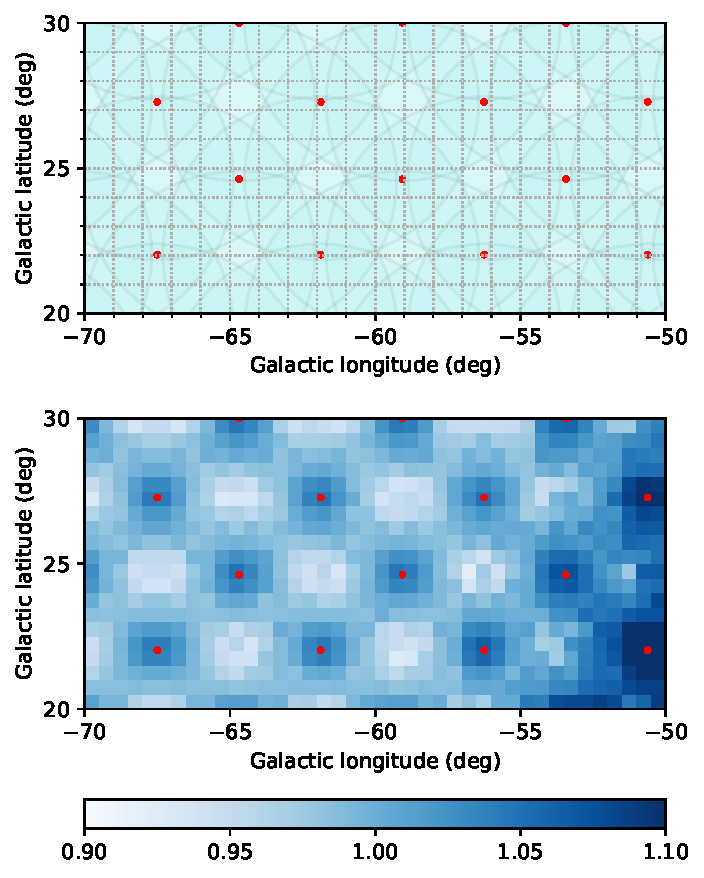
\includegraphics[width=0.45\textwidth]{paper_xcorr/figures/previous_analysis/pointings_zoom20deg_NSIDE16.pdf}
    \caption{Overlapping areas of different pointings. \emph{Top:} A zoomed-in scheme of the pointing strategy shown in \cref{fig:pnts} (red), {together with the overlapping fields of view of individual pointings} (turquoise). \emph{Bottom:} {Simulated exposure map showing variations relative to the average exposure, highlighting the anisotropic pattern created by overlapping pointing regions.}}
    \label{fig:pnt_zoom}
\end{figure}

The IRFs we use are optimized for observations under different zenith angles. {For each pointing direction, we assign one of the three available IRF optimizations based on the minimum zenith angle at which that direction can be observed.} To estimate the minimal zenith angle, we use the Earth coordinates of both array positions, i.e., $(l_N, b_N) = (17.8920, \, 28.7622)$ and $(l_S, b_S) = (79.4041,\, -24.6272)$ for the Northern and Southern array, respectively. The zenith angle is calculated as the angular distance between the array location and the pointing direction when they are closest. The resulting zenith angles for the Northern and Southern arrays are shown in the left panel of \cref{fig:zenith_irf}. The strategy for assigning the IRFs based on zenith angle is adapted from Ref.\ \cite{Remy:2022}. For zenith angles smaller than $30^\circ$, we use the IRF optimized for $20^\circ$ angles; for zenith angles between $30^\circ$ and $50^\circ$ we use the IRF optimized for $40^\circ$ angles, and for zenith angles larger than $50^\circ$ we use IRF optimized for $60^\circ$ angles, as shown in the right panel of \cref{fig:zenith_irf}. All IRFs used in this work are optimized for 5 hours of observation time, independently of the array or the zenith angle.

\begin{figure*}
    \centering
    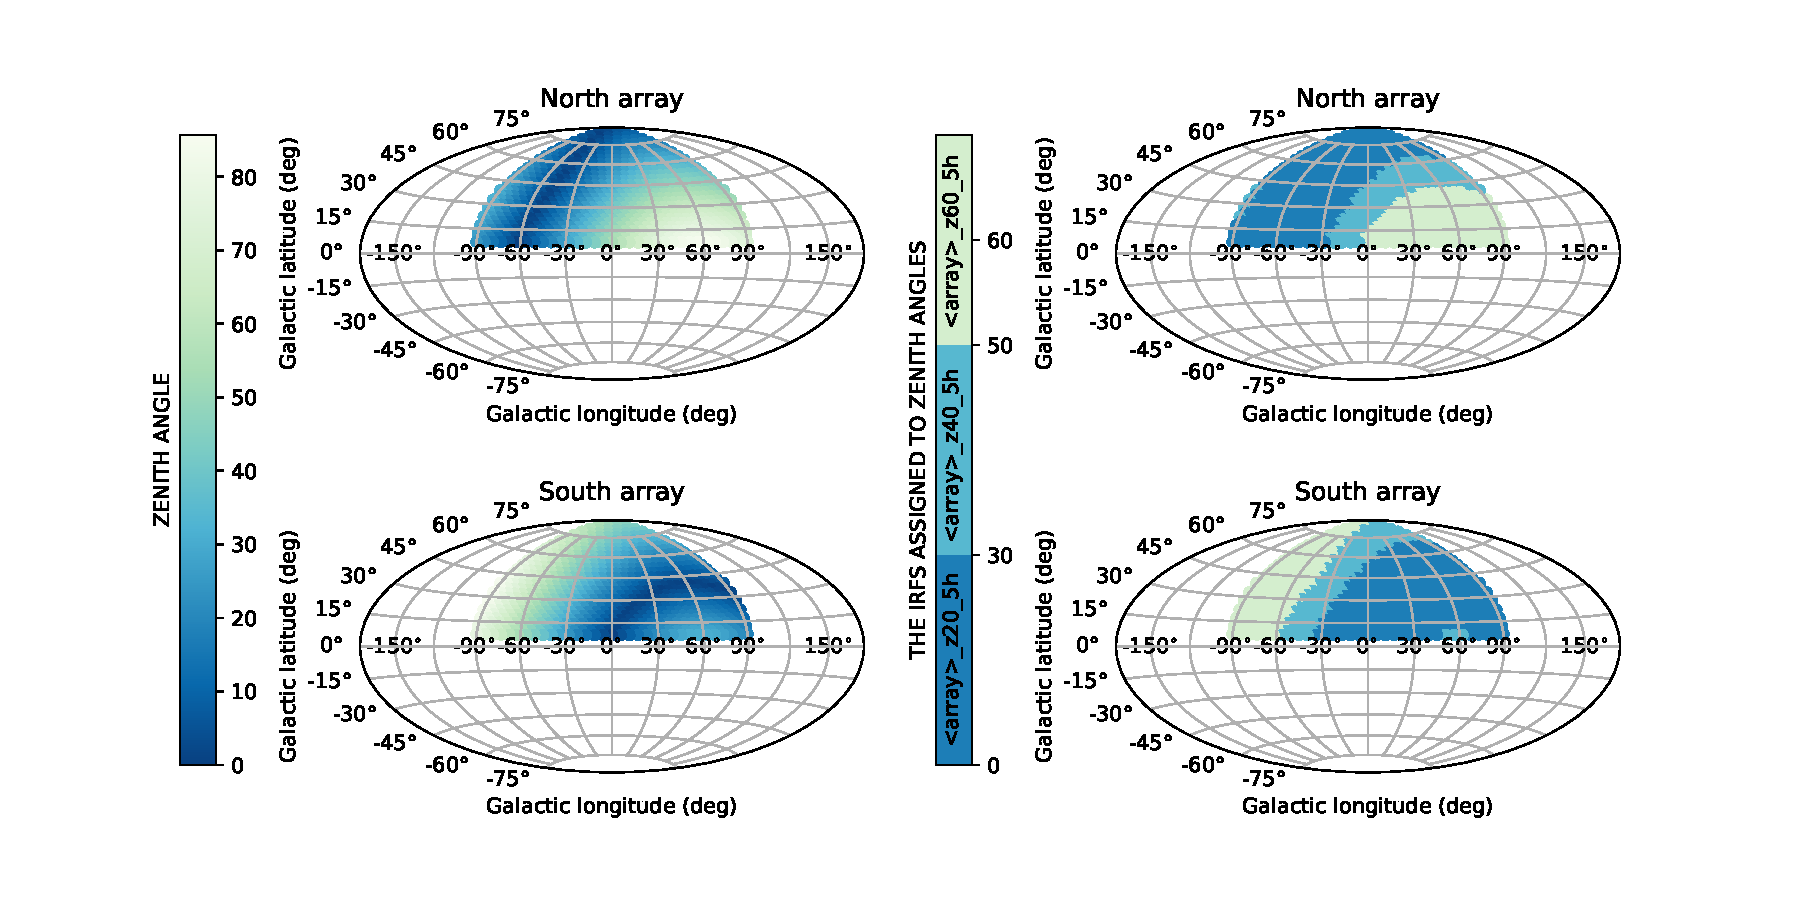
\includegraphics[width=\textwidth]{paper_xcorr/figures/previous_analysis/zenith_angles_NSIDE16_extragal_Luigi_irf5h.pdf}
    \caption{Strategy for assigning Instrument Response Functions (IRFs) across the extragalactic survey region as a function of zenith angle. In the left panel, the color scale shows, for each sky position, the zenith angle as measured in the observatory reference frame during observation (the values of the zenith angles and their color coding are reported on the vertical bar on the left). Since the IRFs are derived in three zenith angle bins (indicated by the color bar on the side of the right panel), the right panel shows which IRF is assigned to each region of the sky. The three IRFs shown here refer to 5 hrs of observation and to zenith angles below 30 deg (dark blue), between 30 and 50 deg (light blue) and above 60 deg (green).
}
    \label{fig:zenith_irf}
\end{figure*}

The observational strategy presented in Section 8 of Ref. \cite{CTAConsortium:2017dvg} divides the extragalactic survey area into two parts: roughly $\sim$15\% of the sky {to be} observed using the Southern array and $\sim$10\% with the Northern array. {However, the precise division of the survey observations between the two arrays has not yet been finalized. The planned strategy remains under discussion and is still subject to adjustments.} For simplicity, we simulate observations of each pointing direction within the survey boundary using both Southern and Northern arrays with the corresponding zenith angle optimized IRFs. We use 1.11 hours and 0.51 hours per pointing direction with the Northern and Southern arrays, respectively. {This strategy provides a reasonable approximation for simulating the survey when combined with zenith-angle–optimized IRFs, as regions observed at higher zenith angles will yield fewer detected events, and vice versa.}  As a result, the sky coverage of both arrays will be complementary, as {illustrated} in the right panel of \cref{fig:zenith_irf}.

The survey observations are simulated for energies between 30 GeV and 30 TeV, using 30 log-spaced energy bins to ensure proper sampling of the IRFs across the energy range. For the purpose of estimating the background events and exposure over the whole extragalactic survey, we simulate the entire survey ROI, using coarser spatial binning of $1.0^\circ \times 1.0^\circ$ per pixel. For the sensitivity analysis, we instead simulate templates covering an ROI of $6.0^\circ\times 6.0^\circ$, using a finer spatial binning of $0.02^\circ \times 0.02^\circ$ per pixel.

\subsubsection{Off-source data scenario}

In addition to performing extensive surveys of the $\gamma$-ray sky, CTAO will be operated as an open, proposal-driven observatory. The observation time awarded to the wider research community can be added to the dedicated survey observation times of CTAO, and increasing the overall exposure that will be achieved over the first 10 years of telescope operation. An educated guess based on the performance of current IACTs can be made for CTAO observations performed through the proposal-driven program. In {Ref.} \cite{Coronado_Blazquez_2021}, the authors calculate the sky coverage and resulting observation time of the CTAO proposal program, assuming similarity with the actual operations of the MAGIC telescope. They extrapolate the 6.5 years of data obtained with the MAGIC array to 10 years of observation time using the two CTAO arrays. We adopt a similar approach to estimate the most optimistic case scenario for the observations of the extragalactic sky with CTAO, assuming an effective observation time of $\sim50$ hours per point and the same sky coverage as in the EGAL survey, consistent with the findings in {Ref.} \cite{Coronado_Blazquez_2021}. In the sensitivity analysis described below, we use a corresponding re-scaling factor to estimate the point source sensitivity of CTAO {under this scenario}. Details on how we derive the effective observation time for this scenario can be found in {\cref{app:expo}}.

